\chapter{Evaluación}
\label{chap:evaluation}

Para llevar a cabo la evaluación del algoritmo se ha hecho uso de la herramienta NVIDIA Nsight Compute. Esta herramienta proporciona un análisis completo sobre la ejecución de un kernel, así como información relevante que puede dar pistas de dónde están los cuellos de botella y que partes conviene optimizar.

Tras crear un proyecto y acceder al perfil de \code{renderingKernel}, el primer dato de relevancia que se ha buscado ha sido que parte del código es la más ejecutada. Conociendo este detalle se puede evitar el esfuerzo de optimizar partes poco relevantes. Para conocer este dato es necesario acceder a la pestaña \code{Source} de la aplicación. En esta pestaña se visualiza el código junto a las instrucciones pptx y a la derecha un mapa de calor que indica en qué partes del código frecuentan más los filtros seleccionados en la pestaña \code{Navigation}.

Se ha seleccionado el filtro de instrucciones ejecutadas donde se han podido localizar dos principales puntos calientes. El primero de los dos es el acceso a los hijos en los nodos del árbol BVH. El segundo es en las funciones de mínimo y máximo. Esto es de esperar ya que son funciones aritméticas que se utilizan en el cálculo de la intersección del rayo con los nodos del árbol.

\begin{figure}[H]
    \centering
	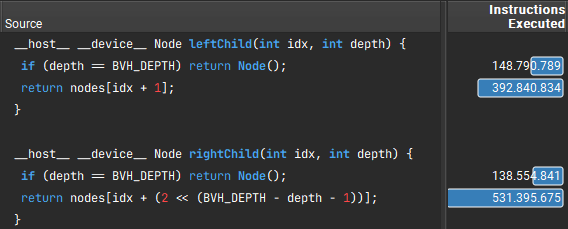
\includegraphics[width=0.5\textwidth]{instructionsexecutedbvh}
	\caption{Nº instrucciones ejecutadas funciones leftChild, righChild}
	\label{fig:label}
\end{figure}

\begin{figure}[H]
    \centering
	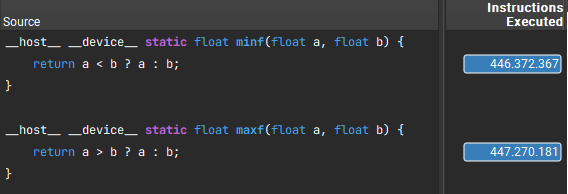
\includegraphics[width=0.5\textwidth]{instructionsexecutedminmax}
	\caption{Nº instrucciones ejecutadas funciones minf/maxf}
	\label{fig:label}
\end{figure}

Estos resultados muestran que la mayoría de las instrucciones ejecutadas se encuentran en el recorrido de los árboles BVH. No es de extrañar que la mayoría de los esfuerzos de optmización del trazado de rayos en el estado del arte residan en estructuras de aceleración más óptimas y compactas. 

NVIDIA Nsight Compute también ofrece advertencias de que partes pueden resultar problemáticas o subóptimas en una arquitectura de GPU en el panel \code{Details}. La ejecución de Eleven Renderer provoca el aviso de un error común en arquitecturas paralelas y es el acceso no secuencial de la memoria. Este fenómeno ocurre cuando los hilos de un wrap no acceden a posiciones contiguas, y en el caso de esta evaluación la advertencia redirige a la parte del código que accede a los hijos del árbol BVH. Esto es de esperar puesto que las estructuras de los árboles no ofrecen buena secuencialidad.

\begin{figure}[H]
    \centering
	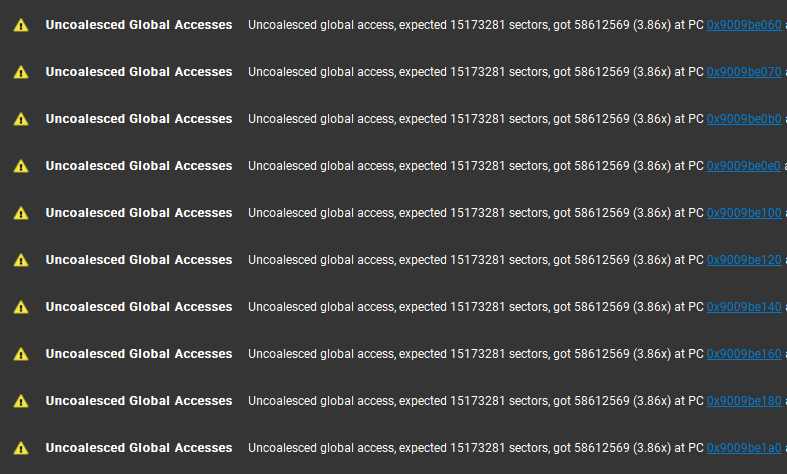
\includegraphics[width=0.5\textwidth]{memoryaccess}
	\caption{Advertencias de acceso no secuencial}
	\label{fig:label}
\end{figure}



\section{Análisis Roofline}
	
El modelo Roofline es utilizado en el análisis de eficiencia de aplicaciones de altas prestaciones. Es un modelo que simplifica la visión del hardware y software mostrando un posible techo de eficiencia. NVIDIA Nsight Compute ofrece este análisis para poder analizar posibles deficiencias y optimizaciones.

La línea superior es una cota superior de 29.23 TFLOPS

El análisis de ejecución de Eleven Renderer para precisión simple\autoref{fig:roofline} ha resultado en 0.36 FLOP/byte de intensidad aritmética y 124.47 GFLOPS de eficiencia, mientras que el techo para una intensidad aritmética de 0.36 FLOP/byte está en 330.65 GFLOPS. Esto indica que el algoritmo está corriendo a un 37.6\% de su capacidad máxima teórica según este modelo siempre y cuando la intensidad aritmética no varíe. Este resultado es razonable, indica que no se está infrautilizando el acelerador gráfico, además indica que el algoritmo tiene una gran dependencia de memoria al encontrarse el punto ubicado muy a la izquierda.

Si se quisiera optimizar más aún este motor, un buen camino sería romper esta dependencia.

\begin{figure}[H]
    \centering
	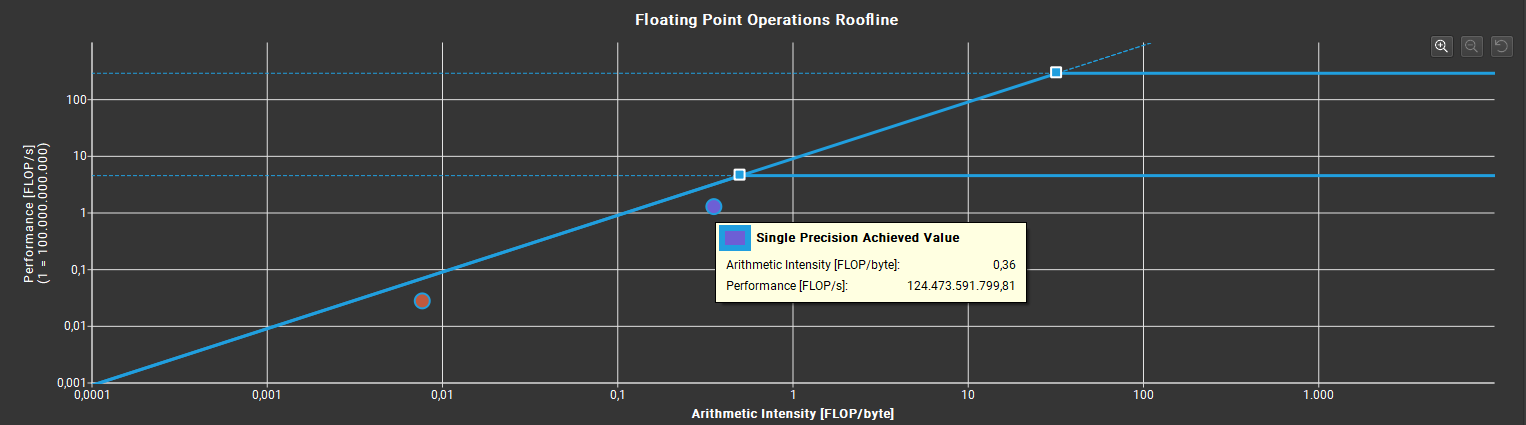
\includegraphics[width=0.5\textwidth]{roofline}
	\caption{Análisis Roofline}
	\label{fig:roofline}
\end{figure}

\chapter{Port oneAPI}
	
oneAPI es un modelo de programación unificado cuyo fin es la implementación de aplicaciones en distintos tipos de aceleradores. 


oneAPI tiene un módulo orientado a la informática gráfica en el que se incluyen herramientas para motores de renderizado. Entre ellas se encuentran Open Image Denoise, una librería que permite renders más detallados con un menor número de muestras gracias al aprendizaje profundo, Embree, que es actualmente el conjunto de kernels más avanzado y eficiente de trazado de rayos gracias a micro optimizaciones adaptadas a distintas arquitecturas, OSPRay, una librería de trazado de rayos y rendering y Open VKL, un kernel de trazado de rayos volumétrico.

Además oneAPI ofrece una plataforma de traducción de código automática que permite convertir código C++ y CUDA a oneAPI. En este capítulo se va a proceder a explicar la conversión realizada de Eleven Renderer, así como los detalles y cambios que han sido necesarios hacer para adaptar esta implementación. También se hará una breve evaluación con el fin de valorar la usabilidad y eficiencia de esta librería y herramienta de portabilidad.

La herramienta en cuestión es DPCT


